\chapter{Gait generation via IS-MPC}
\label{sec:FAPA:GaitGeneration}
The gait generation module receives the planned footstep sequence ${\cal S}_f$ as input, and it is in charge of producing a CoM trajectory that the robot can safely track in order to step over said footstep sequence. Along the entire motion, dynamic balance must be maintained.

On flat ground, it is common to ensure dynamic balance as a geometric criterion, by requiring that the ZMP must always be inside the convex hull of contact surfaces, i.e., the \emph{support polygon}. Traditionally, the ZMP is assumed to be located on the ground plane, which is uniquely defined when the environment is flat.

In non-flat environments, there is no unique ground surface on which the ZMP can be assumed to be. However, the aforementioned criterion can be extended to these cases by allowing the ZMP to move in 3D \cite{SuImYaCa:2021}. The balance criterion is satisfied as long as the ZMP is inside a three-dimensional \emph{support region} $\mathcal{Z}$ that takes the shape of a pyramid (see Fig.~\ref{fig:WoS:balance3d}). The vertex of this pyramid is the robot CoM, and the edges are the lines connecting the CoM to the vertexes of the convex hull of the contact surfaces.

In MPC, dynamic balance is enforced via constraints on the ZMP position. However, the 3D support region $\mathcal{Z}$ cannot be directly employed to enforce a ZMP constraint, because this would be nonlinear, meaning that the resulting optimization problem would not be in a standard linear-quadratic formulation. The cause of this nonlinearity is given by the fact that the vertex of the pyramid $\mathcal{Z}$ is the CoM. Since both the ZMP and the CoM depend on the decision variables of the QP, this would result in product between the decision variables themselves.

In order to avoid this, we will define a smaller region, independent of the CoM position, where the ZMP is allowed to be. Furthermore, we will prove that this region conservatively approximates the actual support region $\mathcal{Z}$, and thus that the balance condition is always satisfied under the imposed constraints.

In this section we will describe the MPC gait generation scheme that is used in the proposed formulation. In particular, we will derive the prediction model and define the constraints that ensure stability and dynamic balance. Finally, we will state the QP problem to be solved at each iteration, and give a sketch of the complete algorithm.

\section{Prediction model}

Control of the ZMP is achieved using a dynamic model relating the position of the latter to the position and acceleration of the CoM. This dynamic model can be derived by balancing moments on the humanoid as a whole, and assuming that the rate of change of angular momentum around the CoM can be neglected, leading to the situtation shown in Fig. \ref{fig:ISMPC:LIPM-robot}, where the Center of Pressure (CoP) is located on the corresponding patch, while the ZMP can be anywhere along the line joining the CoP and the CoM \cite{CaKh:17}.

With this in mind, denoting the CoM as $\bfp_c = (x_c \; y_c \; z_c)^T$ and the ZMP as $\bfp_z = (x_z \; y_z \; z_z)^T$, we get
\begin{equation}\begin{split}
(z_c - z_z)\ddot x_c &= (x_c - x_z)(\ddot z_c + g) \\
(z_c - z_z)\ddot y_c &= (y_c - y_z)(\ddot z_c + g) \\
\ddot{z}_c &= \frac{f_z}{m}-g,
\end{split}\end{equation}
where $g=-9.81$~[m/s$^2$] is the gravity acceleration, $f_z$ denotes the $z$-component of the ground reaction force, acting as an external input, and $m$ is the total mass of the robot.

This model exhibits a nonlinear coupling between the vertical and the horizontal components of $\bfp_c$ and $\ddot\bfp_c$. On flat ground, this nonlinearity is usually handled by assuming a constant CoM height, which leads to the well-known LIP model~\cite{KaKaKaFuHaYoHi:03}. In order to allow for vertical movement of the CoM, a different choice is made here, which is to constrain the motion of the CoM \cite{ZaScLaOr:18} to satisfy the relation
\begin{equation*}
    \frac{\ddot z_c + g}{z_c - z_z} = \eta^2,
\end{equation*}
where $\eta$ is a constant parameter.
The resulting dynamic model can be expressed in the form
\begin{equation}\label{eq:WoS:3dmodel}
\ddot \bfp_c = \eta^2(\bfp_c - \bfp_z) + \bfg,
\end{equation}
where $\bfg = (0 \; 0 \; {g})^T$ is the gravity acceleration vector. This model features a LIP-like dynamic behavior along all three axes. The only difference with respect to a standard LIP is given by the gravity vector $\bfg$ acting as a constant drift. This causes the system not to be in equilibrium when the CoM and ZMP coincide, but rather when they are displaced by $\bfg/\eta^2$.

\begin{figure}
    \centering
    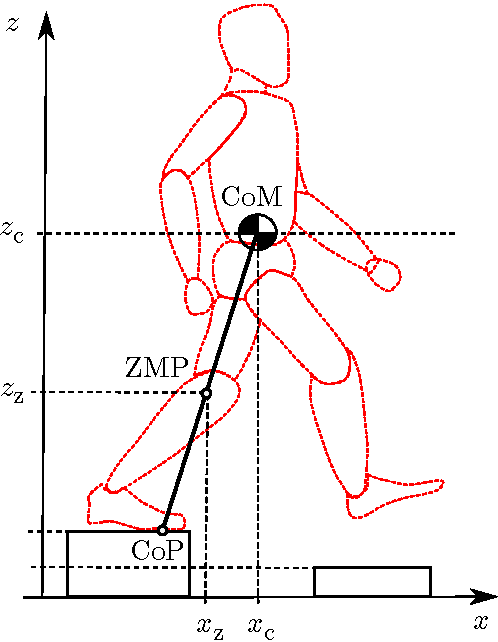
\includegraphics[width=0.4\textwidth]{figures/LIPM_robot.pdf}
    \caption{A humanoid walking on a world of stairs. Note the positions of the CoM, the ZMP and the CoP, which lie on the same axis because of the assumption of conservation of angular momentum.}
    \label{fig:ISMPC:LIPM-robot}
\end{figure}

The choice of restricting the available trajectories to those resulting in a constant $\eta$ allows to make the prediction model linear. If this restriction is removed, the model is referred to as Variable-Height Inverted Pendulum (VH-IP), which can be treated either as nonlinear or time-varying. This can allow for more general motions to be generated, e.g., running~\cite{Smaldone2022Running}, at the cost of a slightly more complex architecture. For the present case, where only walking is considered, the simpler model is preferred.

In order to obtain smoother trajectories, model (\ref{eq:WoS:3dmodel}) is dynamically extended to have the derivative of the ZMP $\dot \bfp_z$ as the input.
The gait generation scheme works over discrete time-steps of duration $\delta$, over which the input $\dot \bfp_z$ is assumed to be constant, i.e.,
\begin{equation*}
    \dot \bfp_z(t) = \dot \bfp_z^k,
\end{equation*}
for $t\in[t_k, t_{k+1})$. This prediction model is used to forecast the evolution of the system over a receding horizon window called the \emph{control horizon}, spanning a time $T_c=C\delta$. The number of steps that are contained, either fully or partially, within this control horizon is denoted as $F$.

\section{Stability constraint}
Model~(\ref{eq:WoS:3dmodel}) has a positive eigenvalue $\eta$, reflecting the intrinsic instability of the humanoid dynamics. Given this instability, it is not sufficient to generate a gait such that the ZMP is inside the support region, because the associated CoM trajectory might be divergent, making the motion unrealizable by the humanoid.
The role of the stability constraint is to enforce a condition on the unstable component of the dynamics in order to guarantee that the CoM trajectory does not diverge with respect to the ZMP.

The unstable component of system (\ref{eq:WoS:3dmodel}) is highlighted by the coordinate
\begin{equation*}
    \bfp_u = \bfp_c + \dot \bfp_c/\eta,
\end{equation*}
also referred to as \textit{divergent component of motion} \cite{EnOtAl:15} or \textit{capture point} \cite{PrCaDrGo:06}, that evolves according to the dynamics
\begin{equation}
\dot\bfp_u = \eta(\bfp_u - \bfp_z) + \frac{\bfg}{\eta}.
\end{equation}
Despite the instability, the evolution of the system is bounded if the following \emph{stability condition} is satisfied
\begin{equation}
\label{eq:WoS:stabilitycondition}
\bfp_u^k = \eta\int_{t_k}^{\infty}e^{-\eta(\tau - t_k)}\bfp_z(\tau) d\tau - \frac{\bfg}{\eta^2},
\end{equation}
where the superscript in ${\bfp}_u^k$ indicates that the variable is sampled at time $t_k$.

Condition~(\ref{eq:WoS:stabilitycondition}) is non-causal as it requires knowledge of the future ZMP trajectory $\bfp_z$ up to infinity. In order to derive a causal implementation, we split the integral at $t_{k+C}$. Of the two separate integrals that result, the first, over $[t_k, t_{k+C})$, can be expressed in terms of the MPC decision variables. A value for the second integral, over $[t_{k+C}, \infty)$, can be obtained by conjecturing a ZMP trajectory using information coming from the footstep plan.
This conjectured trajectory is called \emph{anticipative tail} and is denoted with $\tilde \bfx_z$. 
In \cite{ScDeLaOr:20}, the anticipative tail was used to prove recursive feasibility and stability of the MPC scheme.

The stability constraint is then written as
\begin{equation}\label{eq:WoS:stability_constraint}
\eta\int_{t_k}^{t_{k+C}}e^{-\eta(\tau - t_k)}\bfp_z d\tau = \bfp_u^k - \tilde \bfc^k + \frac{\bfg}{\eta^2}.
\end{equation}
where $\tilde \bfc^k$ is given by
\begin{equation}%\label{eq:WoS:stability_constraint}
\tilde\bfc^k = \eta\int_{t_{k+C}}^{\infty}e^{-\eta(\tau - t_k)}\tilde\bfp_z d\tau.
\end{equation}

Note that \cite{ScDeLaOr:20} considers the footstep plan to be available over a receding window called the \emph{preview horizon}. Here there is no need to make such an assumption, as the footstep plan is provided in its entirety, and once the goal is reached the robot comes to a complete stop.

Enforcing constraint (\ref{eq:WoS:stability_constraint}) allows to bound the displacement between CoM and ZMP. In fact, the value of the bound is almost identical in most practical situation, especially in view of the fact that the preview horizon is unlimited because the plan is completely known.

\textbf{From Humanoids 2023 stability constraint:}
[...] The second step is to make the decision variables appear explicitly, i.e., the ZMP velocities $\dot{\bm{X}}_z$ over the control horizon, by computing the integral over a piecewise linear ZMP trajectory. The final form of the constraint can be found in \cite{ScDeLaOr:20}. For the purpose of this analysis, we will use the compact expression
\begin{equation}\label{eq:FAPA:stability_constraint}
    \bfs^T \dot{\bm{X}}_z = b_x^k + x_u^k,
\end{equation}
where $\bfs\in\mathbb{R}^C$ and $b_x^k\in\mathbb{R}$ denote respectively a vector and a scalar whose explicit expressions can be recovered from the cited reference.


\section{ZMP constraint}
\subsection{Humanoids 2023}
\textbf{From Humanoids 2023 Stability constraint:} Relating the dynamics of the CoM to those of the ZMP is essential since the latter encodes information about the realizability of ground reaction forces, and thus provides a criterion for balance. 
% While on flat ground this criterion consists in keeping the ZMP within the support polygon of the robot, an extension for the 3D case is required. 
A common way to extend the basic 2D balance criterion consists in prescribing the 3D ZMP to be inside a 3D pyramid $\cal Z$ (see Fig.~\ref{fig:FAPA:balance3D}), having the base defined by the contact surfaces and the CoM vertex \cite{Sugihara2002ICRA, Cipriano2023RAS}.

\begin{figure}
    \centering
    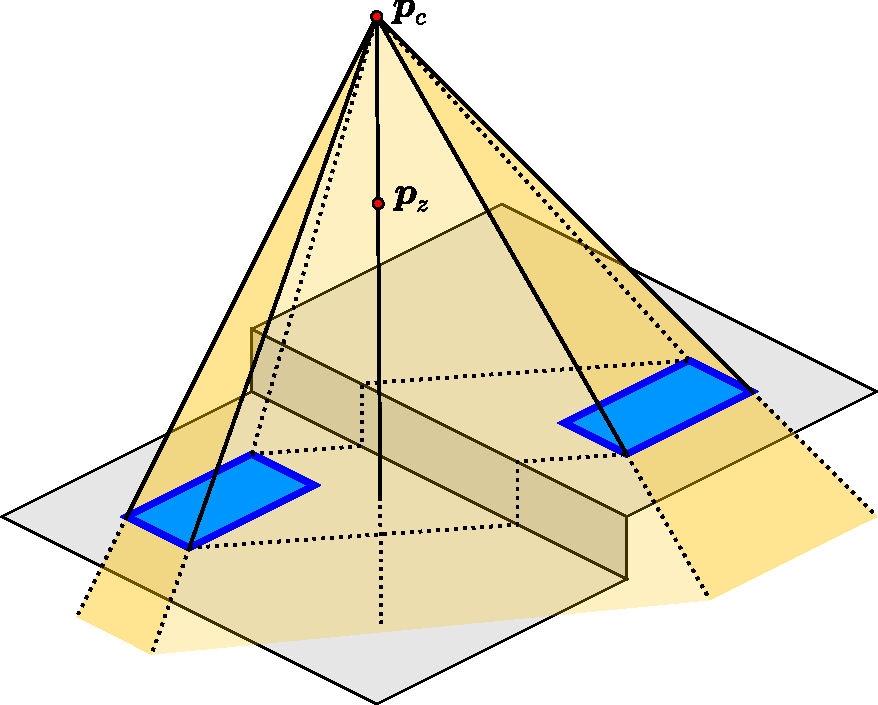
\includegraphics[width=0.55\textwidth]{figures/balance3d.pdf}
    \caption{3D balance: the ZMP $\bfp_z$ must be inside the polyhedral cone $\mathcal{Z}$.}
    \label{fig:FAPA:balance3D}
\end{figure}

The IS-MPC block receives the adapted subplan ${\cal P}^l$ and uses it to construct ZMP constraints. As described in the previous section, the criterion for balance is satisfied if the ZMP belongs to the pyramid $\cal Z$. However, enforcing this condition directly would lead to a nonlinear constraint in the MPC because the vertex of the pyramid is the CoM of the robot. Thus, we adopt a conservative approximation called the {\em moving constraint}.

The moving constraint requires for the ZMP to be at all times within a convex polyhedron of fixed shape, in our case a box of dimensions $d_x$, $d_y$ and $d_z$ centered in $\bfp_{\rm mc}=(x_{\rm mc}, y_{\rm mc}, z_{\rm mc})$, which we call the {\em moving box}. Along the prediction, the moving box can translate but not rotate, and its center moves in such a way that it is always fully contained within the 3D pyramid $\mathcal{Z}$ (see Fig. 5 in \cite{ZaScLaOr:18}). The vector $\bm{X}_{\rm mc}^{k+1} = (x_{\rm mc}^{k+1}, \dots, x_{\rm mc}^{k+C})^T$ collects the $x$ coordinate of the center of the moving box in the control horizon.

Because of its constant orientation in the prediction, at each time we can choose the orientation of the axes to align with the orientation of the moving box (taken as the orientation of the current support foot) and obtain a ZMP constraint that is decoupled along the 3 axes. Focusing on the component along $x$, we can write it as
\begin{equation}\label{eq:FAPA:ZMP_constraints}
    \bm{X}_z^{\rm m,k+1} \le \bm{X}_z^{k+1} \le \bm{X}_z^{M,k+1},
\end{equation}
where $\bm{X}_z^{k+1} = (x_z^{k+1}, \dots, x_z^{k+C})^T$ is a vector of predicted ZMP positions, and $\bm{X}_z^{\rm m,k+1}$ and $\bm{X}_z^{\rm M,k+1}$ are the ZMP bounds along the prediction.
By defining
\begin{equation*}
    \bm{Z} =
    \begin{pmatrix}
        \delta & 0 & \cdots & 0 \\
        \delta & \delta & \cdots & 0 \\
        \vdots & \vdots & \ddots & \vdots \\
        \delta & \delta & \cdots & \delta
    \end{pmatrix},
    \qquad
    \bm{z} =
    \begin{pmatrix}
        1 \\ 1 \\ \vdots \\ 1
    \end{pmatrix},
\end{equation*}
$\bm{X}_z^{k+1}$ can be expressed as
\begin{equation}
    \label{eq:FAPA:zmp-model-matrix-form}
    \bm{X}_z^{k+1} = \bm{Z} \dot{\bm{X}}_z^{k} + \bm{z} x_z^k,
\end{equation}
where $\dot{\bm{X}}_z^{k} = (\dot x_z^{k}, \dots, \dot x_z^{k+C-1})^T$ is the vector of ZMP velocities, i.e., the decision variables. The ZMP bounds along the prediction can be expressed as
\begin{equation}
    \bm{X}_z^{\rm m,k+1} = \bm{X}_{\rm mc}^{k+1} - \bfz \frac{d_x}{2}, \quad 
    \bm{X}_z^{\rm M,k+1} = \bm{X}_{\rm mc}^{k+1} + \bfz \frac{d_x}{2}.
\label{eq:FAPA:zmp_constraint_displacement}
\end{equation}
The center of the moving box $\bfp_{\rm mc}$ must be expressed in terms of the subplan $\mathcal{P}^l$. First we define the {\em piecewise-linear sigmoid} function 
\begin{equation*}
\sigma (t,t_i,t_f)=\frac{1}{t_f-t_i} \left(\rho(t-t_i)-\rho(t-t_f)\right),
%\label{eq:FAPA:sigma}
\end{equation*}
where $\rho(t)=t\delta_{-1}(t)$ is the unit ramp. $\sigma (t,t_i,t_f)$ is 0 before $t_i$,  1 after $t_f$, and it transitions linearly in the interval $[t_i,t_f]$. This function is useful to represent the transition between consecutive footsteps.

$\bm{X}_{\rm mc}^{k+1}$ can be written as
\begin{equation}
\label{eq:FAPA:mapping}
\bm{X}_{\rm mc}^{k+1} = \bm{M} \bm{X}_f^l + \bm{m}x_f^l,
\end{equation}
where $\bm{X}_{f}^{l} = (x_{f}^{l}, \dots, x_{f}^{l+F})^T$ collects the footstep positions. $\bm{M}\in\mathbb{R}^{C\times F}$ is a mapping matrix whose elements $M_{ij}$ are defined as
\begin{equation}\begin{split}
M_{ij} &= \sigma(t_{k+i}, t_s^{l+j},t_s^{l+j}+T_{\rm ds}^{l+j})\\ &- \sigma(t_{k+i}, t_s^{l+j-1},t_s^{l+j-1}+T_{\rm ds}^{l+j-1}),
\end{split}\end{equation}
and $\bfm\in\mathbb{R}^{C}$ is a vector whose elements $m_i$ are given by
\begin{equation*}
m_{i} = 1 - \sigma(t_{k+i}, t_s^{l},t_s^{l}+T_{\rm ds}^{1}),
\end{equation*}
where $t_s^l$ is the starting time of the $l$-th step and
\begin{equation*}
    t^j_s = t^l_s + \sum^{l+j-1}_{\lambda=l} \left(T_{\rm ds}^\lambda + T_{\rm ss}^\lambda\right).
\end{equation*}

\subsection{RAS 2023}
As already noted, the humanoid is balanced as long as the ZMP is inside the pyramid $\cal Z$, which is a nonlinear condition due to the vertex of the pyramid being at the CoM (Fig. \ref{fig:WoS:balance3d}). To preserve linearity we consider a smaller allowed region for the ZMP, consisting in a box of fixed size with changing center and orientation. We refer to this as the {\em moving box}\footnote{Approximating the pyramidal region $\cal Z$ with a box might seem overly conservative. However, we argue that the neglected portion of the pyramid region is not crucial here, because large displacements of the ZMP in the $z$ direction would only be required to generate large vertical accelerations, which are not necessary in the considered setting (walking in a world of stairs). Clearly, less conservative approximations can still be envisaged and used for generating more dynamic motions.}, and we will prove that it conservatively approximates the support region, meaning that it is always contained inside the pyramid $\cal Z$.



%However, we argue that the neglected portion of the pyramid region is not crucial here, because large displacements of the ZMP in the $z$ direction are only required to generate large vertical accelerations, which are not necessary in the considered setting (walking in a world of stairs).



\begin{figure}
    \centering
    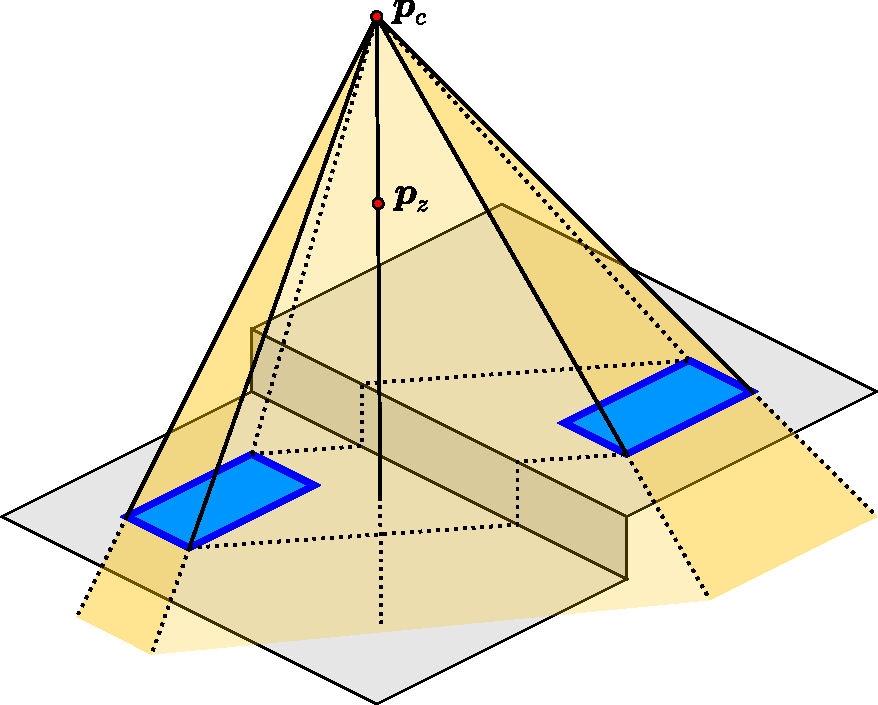
\includegraphics[width=0.6\textwidth]{figures/balance3d.pdf}
    \caption{Balance condition in 3D: the ZMP must lie inside the yellow pyramid.}
    \label{fig:WoS:balance3d}
\end{figure}

The center $\bfp_{\rm mc}$ and orientation $\theta_{\rm mc}$ of the moving box are taken to be consistent with the pose of footstep $\bff^j$ during the $j$-th single support phase. In the following double support phase they will gradually slide in order to reach the pose of the next footstep $\bff^{j+1}$, with a linear\footnote{The timing law can be arbitrarily chosen as long as it leads the moving box from one footstep to the next within the duration of the double support phase.} timing law. At each time $t$, the center of the moving box $\bfp_{\rm mc}$ is expressed as
\begin{equation}\label{eq:WoS: moving constraint}
\bfp_{\rm mc}(t) = \Bigg\{
\begin{array}{ll}
\bfp^j & t\in [t_s^j, t_s^j + T_{\rm ss}^j) \\
(1-\alpha^j(t))\bfp^j + \alpha^j(t)\bfp^{j+1} & t\in [t_s^j + T_{\rm ss}^j, t_s^{k+1})
\end{array}
\end{equation}
where $j=0,\dots,F$ is a index over the footsteps within the control horizon, and $\alpha^j(t) = (t-t_s^j-T_{\rm ss}^j)/T_{\rm ds}^j$ denotes the time elapsed since the start of the double support phase, expressed as a fraction of the duration of the double support phase itself.
The orientation of the moving box $\theta_{\rm mc}$ can be similarly expressed as
\begin{equation}\label{eq:WoS: moving constraint angle}
\theta_{\rm mc}(t) = \Bigg\{
\begin{array}{ll}
\theta^j & t\in [t_s^j, t_s^j + T_{\rm ss}^j) \\
\mathrm{anglin}(\theta^j,\theta^{j+1},\alpha^j(t)) & t\in [t_s^j + T_{\rm ss}^j, t_s^{k+1})
\end{array}
\end{equation}
where $j=0,\dots,F$, and $\mathrm{anglin}$ is a function\footnote{For two generic angles
$\theta_a$ and $\theta_b$, linearly combined with a weight $\alpha$, the function $\mathrm{anglin}$ can be defined as
\begin{equation*}\begin{split}
\mathrm{anglin}(\theta_a, \theta_b, \alpha) = \mathrm{atan2}(&\sin((1-\alpha)\theta_a) + \sin(\alpha\theta_b), \\&\cos((1-\alpha)\theta_a) + \cos(\alpha\theta_b)).
\end{split}\end{equation*}
Note that this definition is meaningless when the two angles are separated by exactly $\pi$, but this can never occur as the angle between consecutive footsteps is limited by requirement R2. } that computes a linear combination of angles in such a way to correctly account for wrapping around $\pm\pi$.

The ZMP position constraint is expressed as
\begin{equation}\label{eq:WoS:ZMP_constraint}
-\tilde\bfd /2 \le \bfR_{k+i}^T(\bfp_z^{k+i} - \bfp_{\rm mc}^{k+i}) \le \tilde\bfd /2
\end{equation}
where $\bfp_z^{k+i}$ and $\bfp_{\rm mc}^{k+i}$ respectively denote the ZMP and the center of the moving box sampled at time $t_{k+i}$, $\tilde \bfd = (\tilde d_x, \tilde d_y, d_z)^T$
is a vector collecting the dimensions of the moving box along all three axes, and $\bfR_{k+i}$ is the rotation matrix associated with $\theta_{\rm mc}^{k+i}$.

The size of the moving box $\tilde \bfd = (\tilde d_x, \tilde d_y, d_z)^T$ is determined in such a way to always be contained inside the pyramid $\cal Z$



\section{IS-MPC algorithm}
\subsection{Humanoids 2023}
IS-MPC solves, at each time $t_k$, the following QP problem:
\begin{braced}
\begin{equation*}\begin{split}
\min_{\dot{\bm{X}}_\text{z}^k, \dot{\bm{Y}}_\text{z}^k, \dot{\bm{Z}}_\text{z}^k}
&\|\dot{\bm{X}}_z^k\|^2 + \|\dot{\bm{Y}}_z^k\|^2 + \|\dot{\bm{Z}}_z^k\|^2+\beta \|\bm{X}_z^{k+1} - \bfX_{\rm mc}^{k+1}\|^2 \\& + \beta \|\bm{Y}_z^{k+1} - \bfY_{\rm mc}^{k+1}\|^2 + \beta \|\bm{Z}_z^{k+1} - \bfZ_{\rm mc}^{k+1}\|^2 \\
\end{split}\end{equation*}
\hspace{0.25cm} subject to:
\begin{itemize}
\item ZMP constraints (\ref{eq:FAPA:ZMP_constraints})
\item stability constraints (\ref{eq:FAPA:stability_constraint})
\end{itemize}
\end{braced}

In the cost function, the first three terms act as regularization while the remaining attempt to bring the ZMP as close as possible to the center of the moving box, with a strength modulated by the weight $\beta$.

The first sample $\dot \bfp_z^k = (\dot x_z^k, \dot y_z^k, \dot z_z^k)$ of the optimal sequence is used to integrate the prediction model and the resulting CoM position $\bfp_c^{k+1}$ is sent to the kinematic controller together with a suitable swing foot trajectory that allows to reach the target footstep position at the proper time.

\subsection{RAS 2023}
At a generic time $t_k$, IS-MPC solves the following QP problem

\begin{braced}
\[
\min_{\dot \bfp_z^k, \dots, \dot \bfp_z^{k+C-1}} \quad \sum_{i=0}^{C-1} \left(\|\dot\bfp_z^{k+i}\|^2 + \beta\|\bfp_z^{k+i} - \bfp_{\rm mc}^{k+i}\|^2\right)
\]
\hspace{0.25cm} subject to:
\begin{itemize}
\item stability constraint (\ref{eq:WoS:stability_constraint})
\item ZMP position constraint (\ref{eq:WoS:ZMP_constraint})
\end{itemize}
\end{braced}
The cost function minimizes the decision variables (ZMP derivative) as a regularization term, and attempts to bring the ZMP close to the center of the moving box, which is typically beneficial as it produces a more robust walking pattern. $\beta$ is a weight on the second term.

In typical MPC fashion, the first sample of the ZMP velocity $\dot \bfp_z^k$ is used to integrate the 3D LIP dynamics (\ref{eq:WoS:3dmodel}). The resulting CoM trajectory $\bfp_c$ is sent, together with the swing foot trajectory generated by the footstep planner and sampled at time $t_k$, to the kinematic controller.


\section{Feasibility region}

The {\em feasibility region} is the region of the state space in which the IS-MPC optimization problem is feasible.

\begin{proposition}
\label{prop:feasibility}
IS-MPC is feasible at time $t_k$ if
\begin{align}
\label{eq:FAPA:mpc-feasibility-constraint}
\bm{s}^T \bm{Z}^{-1} (\bm{X}_z^{{\rm m}, k+1} \!-\! \bm{z} x_z^k)  \!&\le\! x_u^k \!+\! b_x^k \!\le\! \bm{s}^T \bm{Z}^{-1} (\bm{X}_z^{{\rm M}, k+1} \!-\! \bm{z} x_z^k),
\nonumber\\
\bm{s}^T \bm{Z}^{-1} (\bm{Y}_z^{{\rm m}, k+1} \!-\! \bm{z} y_z^k)  \!&\le\! y_u^k \!+\! b_y^k \!\le\! \bm{s}^T \bm{Z}^{-1} (\bm{Y}_z^{{\rm M}, k+1} \!-\! \bm{z} y_z^k),
\nonumber\\
\bm{s}^T \bm{Z}^{-1} (\bm{Z}_z^{{\rm m}, k+1} \!-\! \bm{z} z_z^k)  \!&\le\! z_u^k \!+\! b_z^k \!\le\! \bm{s}^T \bm{Z}^{-1} (\bm{Z}_z^{{\rm M}, k+1} \!-\! \bm{z} z_z^k).
\end{align}
\end{proposition}
{\em Proof}.
We focus the proof on the inequalities for the $x$ component, as the logic, for the other components is identical. The bounds of the feasibility region along $x$ are given by
\begin{align*}
x_u^{k,b1} &= \bm{s}^T \bm{Z}^{-1} (\bm{X}_z^{{\rm m}, k+1} - \bm{z} x_z^k) - b_x^k, \\
x_u^{k,b2} &= \bm{s}^T \bm{Z}^{-1} (\bm{X}_z^{{\rm M}, k+1} - \bm{z} x_z^k) - b_x^k.
\end{align*}
Then, if $x_u^k$ is inside the feasibility region, it is possible to express it as a convex combination of the two bounds, i.e.,
\begin{equation}\label{eq:FAPA:xu_convex}
x_u^k = \alpha x_u^{k,b1} + (1-\alpha)x_u^{k,b2}, \alpha \in [0, 1].
\end{equation}

Consider the following ZMP velocity trajectory:
\begin{equation}\label{eq:FAPA:candidate_trajectory}
\dot{\bm{X}}_z^k = \alpha \bm{Z}^{-1}(\bm{X}_z^{{\rm m}, k+1} - \bm{z} x_z^k) + (1-\alpha)\bm{Z}^{-1}(\bm{X}_z^{{\rm M}, k+1} - \bm{z} x_z^k).
\end{equation}
We will show that this particular trajectory satisfies both the stability constraint and the ZMP constraints. As for the stability constraint, multiply both sides of (\ref{eq:FAPA:candidate_trajectory}) by $\bm{s}^T$
% \begin{equation}
% \bm{s}^T\bm{\dot X}_z^k = \bm{s}^T(\alpha \bm{Z}^{-1}(\bm{X}_z^{{\rm m}, k+1} - \bm{z} x_z^k) + (1-\alpha)\bm{Z}^{-1}(\bm{X}_z^{{\rm M}, k+1} - \bm{z} x_z^k)),
% \end{equation}
and plug in the definitions of $x_u^{k,b1}$ and $x_u^{k,b2}$ to obtain
\begin{equation*}
\bm{s}^T\dot{\bm X}_z^k = (\alpha (x_u^{k,b1} + b^k_x)) + (1-\alpha)(x_u^{k,b2} + b^k_x)).
\end{equation*}
Using (\ref{eq:FAPA:xu_convex}), this is equivalent to the stability constraint (\ref{eq:FAPA:stability_constraint}).

To prove satisfaction of the ZMP constraint. Left-multiplying \eqref{eq:FAPA:zmp-model-matrix-form} by $\bm{Z}$, the chosen ZMP velocity trajectory can be rewritten as
\begin{equation*}
\bm{X}_z^k - \bm{z} x_z^k = \alpha (\bm{X}_z^{{\rm m}, k+1} - \bm{z} x_z^k) + (1-\alpha)(\bm{X}_z^{{\rm M}, k+1} - \bm{z} x_z^k),
\end{equation*}
which simplifies to
$\bm{X}_z^k = \alpha \bm{X}_z^{{\rm m}, k+1} + (1-\alpha)\bm{X}_z^{{\rm M}, k+1}$,
and therefore the ZMP constraint (\ref{eq:FAPA:ZMP_constraints}) is satisfied. \hfill\bull

In the following section, we will describe how to use the feasibility region to formulate a constraint for the FAPA module, and thus ensure that the output of FAPA can be used by IS-MPC to construct a feasible QP.
